%% Latex Template for MSc projects - Deliverable I
%% School of Science, Computer Science Department
%% Loughborough University
%% Prepared by Andrea Soltoggio, 2018

\documentclass[12pt,oneside,a4paper]{article}
\usepackage[utf8]{inputenc}
\usepackage[english]{babel}
\usepackage{fancyhdr}
\usepackage{graphicx}
\usepackage{natbib}

\usepackage[hyphens]{url}
\usepackage[hidelinks]{hyperref}
\hypersetup{breaklinks=true}
\urlstyle{same}
\usepackage{booktabs}

%\setlength{\arrayrulewidth}{1mm}
\setlength{\tabcolsep}{6pt}
\renewcommand{\arraystretch}{1.5}

\renewcommand{\baselinestretch}{1.15}

%----------------------------------------------------------------------------------------
%	TITLE PAGE
%----------------------------------------------------------------------------------------

% Create the command for including the title page with \makeTatlePage command
\newcommand*{\makeTitleParagraph}{
\begingroup
\begin{center}

\includegraphics[width = 7cm]{LoughboroughLogo.png} \par
COP324 - Project preparation\par
Deliverable I. \par
\end{center}

 
\noindent


\noindent
\textbf{Title of the project:} AI Assisted Bone Fracture Detection and Localization from Multi-view X-Ray Images\\ 
\textbf{Name:} Weipeng Wu\\
\textbf{Student ID: B836051}\\
\textbf{Supervisor:} Dr. Lianghao Han\\
\textbf{Programme:} Advanced Computer Science\\
\textbf{Submitted:} $1^{th}$ April 2020\\
\endgroup}

%----------------------------------------------------------------------------------------
%	DOCUMENT
%----------------------------------------------------------------------------------------

\begin{document}

\makeTitleParagraph % This command includes the title page

\paragraph{Abstract.} Artificial intelligence (AI) is developing remarkable progress in clinical diagnosis and even amount of researchers have devoted to this filed for making more contributions. however, more advanced models and methods still should be improved by using deep learning, such as detecting bone fracture automatically or determine the possibility of cancer for the patients by using deep learning methods. In this paper, we proposed a novel and high effective method to implement the fracture detection for the various human bones. This method can annotate the images obtained from MURA dataset automatically and detect whether the bone fracture happens or not by using the improved model based on Faster R-CNN and other models. Meanwhile, this method results will compare with the judgement of the radiologists and orthopedists.
%\end{abstract}

\section{Introduction}
The clinical diagnosis is used for detecting all kinds of

\section{Aims and Objectives}
\section{Main and Methodology}
\section{Project Plan}
\section{Reference}
\subsection{This is a subsection}

\subsection{Tables and Figures}

Figure \ref{fig.niceFigure} is an example of a figure.
\begin{figure}
\begin{center}
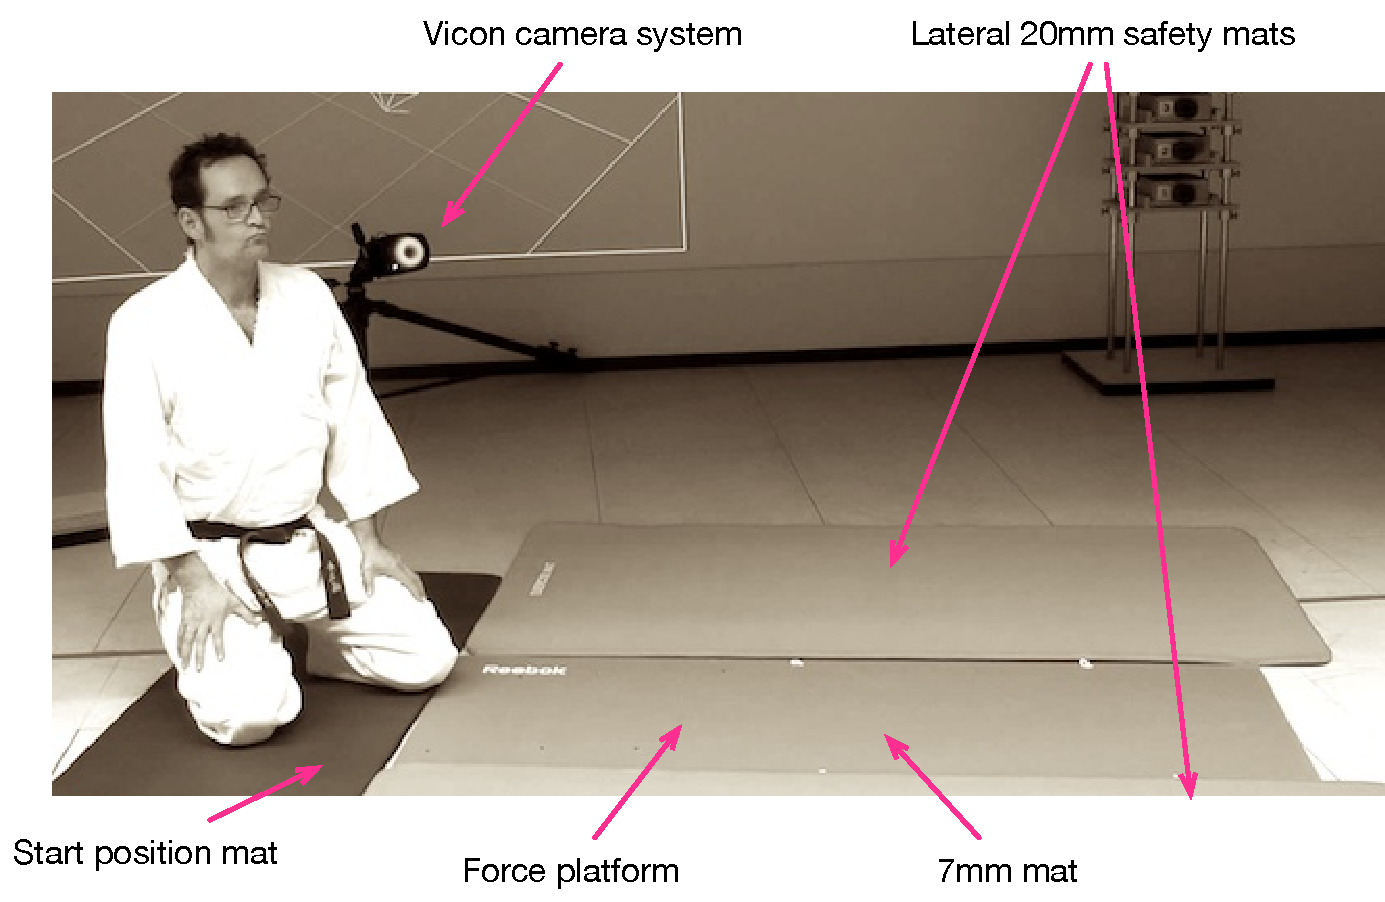
\includegraphics[width=0.6\columnwidth]{f2_expSetup}
\caption{Here goes the caption of the figure.}
\label{fig.niceFigure}
\end{center}
\end{figure}

Here we show some numbers in Table \ref{tab.someTable}


\begin{table}
\begin{center}
\begin{tabular}{|p{3cm}|p{3cm}|p{3cm}|p{3cm}|}
\hline
\multicolumn{4}{|c|}{Country List} \\
\hline
Country Name     or Area Name& ISO ALPHA 2 Code &ISO ALPHA 3 Code&ISO numeric Code\\
\hline
Afghanistan   & AF    &AFG&   004\\
Aland Islands&   AX  & ALA   &248\\
Albania &AL & ALB&  008\\
Algeria    &DZ & DZA&  012\\
American Samoa&   AS  & ASM&016\\
Andorra& AD  & AND   &020\\
Angola& AO  & AGO&024\\
\hline
\end{tabular}
\label{tab.someTable}
\caption{Here is the caption of the table}\vspace{8pt}
\end{center}
\end{table}

\subsection{Equations}

Equation \ref{eq.PDI} is an example of a nice equation.
\begin{equation}
\frac{\partial O}{\partial I_{i}} = \sum_{j}{\frac{\partial O}{\partial h_{j}}\frac{\partial h_{j}}{\partial S_{j}^{1}}\frac{\partial S_{j}^{1}}{\partial I_{i}}}\quad.
\label{eq.PDI}
\end{equation}
As equation \ref{eq.PD2ndO} shows, there is no limit to your fantasy when it comes to writing equations.
\begin{eqnarray}
\nonumber\frac{\partial^{2} O}{\partial I_{i}^{2}} =
\sum_{j}w_{ij}^{0}\Bigg [ (1 - 2h_{i})h_{j}(1 - h_{j})w_{ij}^{0}\frac{\partial O}{\partial h_{j}} +\\
+ h_{j}(1 - h_{j})\Bigg(\frac{\partial^{2} O}{\partial I_{i} \partial h_{j}}\Bigg)
\Bigg ]\label{eq.PD2ndO}
\end{eqnarray}

\subsection{Citing}

Insert references in the bibtex file using the bibtex format. Latex makes sure that references are displayed correctly. Make sure you use journal papers, books and conferences papers predominantly. These are authoritative, peer-reviewed sources. Webpages can be occasionally cited, but are considered as less authoritative.
the ski

Typically, when you make a statement that is substantiated by information in a source document, you are require to cite the source \citep{bullinaria2009}. Sometimes more sources substantiate your statement \citep{soltoggioSteilNeuralComputation2013,soltoggioHTP2014}. 

Sometimes you want to use a citation as subject of your sentence. For example, \citet{SuttonBarto1998} introduce basic concepts in reinforcement learning.



\bibliographystyle{apalike}
\bibliography{MyBibliography}

\end{document}